\section{实验一:填充文本}

填充文本填充文本填充文本填充文本填充文本填充文本填充文本填充文本填充文本填充文本填充文本填充文本填充文本填充文本填充文本填充文本填充文本填充文本。图表引用如:见图 \ref{plot_random_points}。

\begin{figure}[htbp]
    \centering
    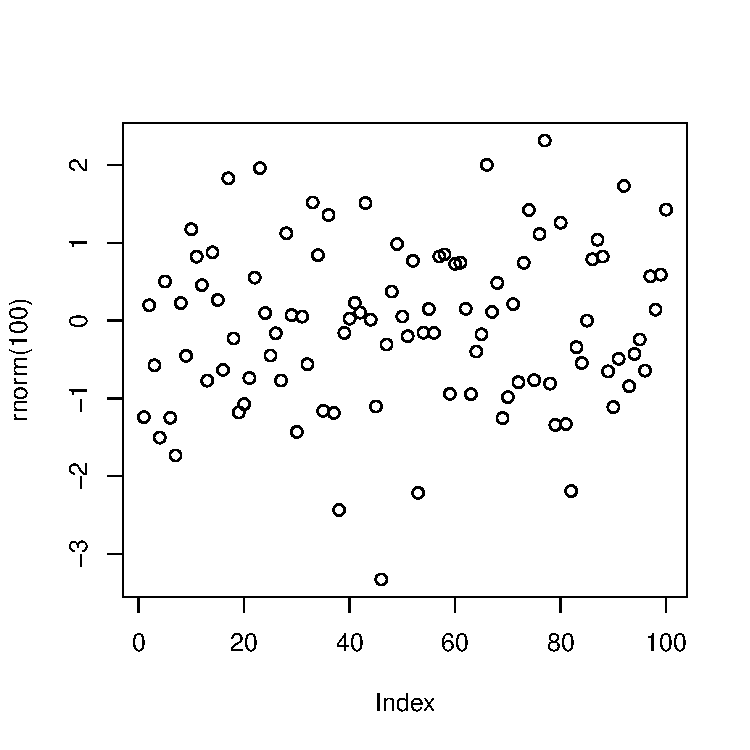
\includegraphics[width=0.5\linewidth]{Pictures/Exp1/plot_random_points.pdf}
    \caption{100 个正态分布的随机数}
    \label{plot_random_points}
    \notefig{100 个正态分布的随机数。填充文本填充文本填充文本填充文本填充文本填充文本填充文本填充文本填充文本填充文本填充文本填充文本填充文本填充文本填充文本填充文本填充文本填充文本。}
\end{figure}

填充文本填充文本填充文本填充文本填充文本填充文本填充文本填充文本填充文本填充文本填充文本填充文本填充文本填充文本填充文本填充文本填充文本填充文本。表格引用如:见表 \ref{table_fit}。

\begin{table}
    \centering
    \begin{threeparttable}
        \caption{填充文本填充文本}
        \label{table_fit}
        \begin{tabular*}{0.9\textwidth}{l @{\extracolsep{\fill}} r r c r r @{\extracolsep{0cm}} @{} l}
            \toprule
            & \multicolumn{1}{c}{$b$} & \multicolumn{1}{c}{SE} & \multicolumn{1}{c}{95\% CI} & \multicolumn{1}{c}{df} & \multicolumn{2}{c}{$t$} \\
            \midrule
            填充文本      &  1.11  &  1.11  & $(1.11, 2.22)$ &  11  &  11.11  &  $^{***}$  \\
            填充文本  &  1.11  &  1.11  & $(1.11, 2.22)$ &  11  &  11.11  &  $^{**}$  \\
            填充文本  &  1.11  &  1.11  & $(1.11, 2.22)$ &  11  &  11.11  &  $^{*}$  \\
            填充文本  &  1.11  &  1.11  & $(1.11, 2.22)$ &  11  &  11.11  &  $^{\dagger}$\\
            \bottomrule
        \end{tabular*}
        \notetable{填充文本填充文本填充文本填充文本填充文本填充文本填充文本填充文本填充文本填充文本填充文本填充文本填充文本填充文本填充文本填充文本填充文本填充文本。\\
        $^{***} p < 0.001; \quad ^{**} p < 0.01; \quad ^{*} p < 0.05; \quad ^{\dagger} p < 0.1$}
    \end{threeparttable}
\end{table}

填充文本填充文本填充文本填充文本填充文本填充文本填充文本填充文本填充文本填充文本填充文本填充文本填充文本填充文本填充文本填充文本填充文本填充文本。

\begin{sidewaysfigure}
    \centering
    \begin{tikzpicture}
        \node at(0, 0) [mynode] (x) {起始点};
        \node at(7, 0) [mynode] (m1) {中间点一};
        \node at(13, 1.5) [mynode] (m2) {中间点二};
        \node at(13, -1.5) [mynode] (m3) {中间点三};
        \node at(19, 0) [mynode] (y) {终点};

        \draw[-latex] (x.east) -- node[above, font=\footnotesize, align=left]{$a_1 = 1.11^{*}$ \\ $a_2 = 1.11^{*}$} (m1.west);

        \draw[-latex] (m1.east) -- (m2.west);
        \draw (10, 1.3) node[font=\footnotesize]{$m_1 = -1.11^{*}$};
        \draw[-latex] (m1.east) -- (m3.west);
        \draw (10, -1.3) node[font=\footnotesize]{$m_2 = -1.11^{*}$};

        \draw[-latex] (m2.east) -- (y.west);
        \draw (16, 1.2) node[font=\footnotesize]{$b_1 = 1.11^{*}$};
        \draw[-latex, dashed] (m3.east) -- (y.west);
        \draw (16, -1.2) node[font=\footnotesize]{$b_2 = 1.11$};

        \draw[-latex] (x.south) -- (0, -3) -- (19, -3) -- (y.south);
        \draw (7, -2.2) node[font=\footnotesize, align=left]{$c'_1 = 1.11^{*}$ \\ $c'_2 = 1.11^{*}$};
        \draw (7, -3.8) node[font=\footnotesize, align=left]{$c_1 = 1.11^{*}$ \\ $c_2 = 1.11^{*}$};
    \end{tikzpicture}
    \caption{TikZ 绘图示例}
    \label{plot_flow}
    \notefig{填充文本填充文本填充文本填充文本填充文本填充文本填充文本填充文本填充文本填充文本填充文本填充文本填充文本填充文本填充文本填充文本填充文本填充文本。}
\end{sidewaysfigure}



